\documentclass[a4paper,10pt]{article}

\usepackage[utf8]{inputenx}
\usepackage[style=apa,backend=biber,alldates=iso8601]{biblatex}
\usepackage[nottoc,notlot,notlof]{tocbibind}
\usepackage[font={it}, labelfont=bf]{caption}
\usepackage{hyperref}
\usepackage[braket, qm]{qcircuit}
\usepackage{a4wide}
\usepackage{enumitem}
\usepackage{fancyhdr}
\usepackage{blochsphere}
\usepackage{xcolor}
\usepackage{amssymb}
\usepackage{amsmath}
\usepackage{multirow}
\usepackage{subcaption}
\usepackage{multicol}
\usepackage{dirtytalk}
\usepackage{tikz-3dplot}
\usepackage[outline]{contour}
\usetikzlibrary{3d}

\DeclareLanguageMapping{english}{english-apa}
%\DeclareFieldFormat[article,unpublished,misc,online]{title}{\textit{#1}}

\renewcommand{\abstractname}{Summary}
\renewcommand*{\bibfont}{\small}

\DeclareMathOperator{\sign}{sign}

\newcommand{\qstatezero}{
	\begin{pmatrix}1 \\ 0\end{pmatrix}
}
\newcommand{\qstateone}{
	\begin{pmatrix}0 \\ 1\end{pmatrix}
}

\newcommand{\hgate}{
	\dfrac{1}{\sqrt2}
	\begin{pmatrix}
		1 & \phantom{-}1 \\
		1 & -1
	\end{pmatrix}
}

\addbibresource{quantum-internship-research-paper.bib}

\title{Simulation of Quantum Algorithms for Solving Machine Learning Problems}
\author{Steven Oud \\ \emph{SURFsara, Amsterdam}}
\date{\today}

\begin{document}

\maketitle

\begin{abstract}
Quantum computing is a promising technology of the near future.
Since its first proposal researchers have been looking to use it for solving difficult chemistry and physics problems.
More recently, research towards its application in the field of machine learning has shown promise.
We take a look at how to apply current state-of-the-art quantum algorithms to solve machine learning problems.
With the help of quantum circuit simulation we implement a variational quantum neural network for classifying handwritten digits and demonstrate that a QNN can be trained to perform binary, one-vs-rest and multiclass classification.
\end{abstract}

\tableofcontents

\clearpage

\section{Introduction}
Quantum computing is one of the most promising technology developments of the coming years.
Big companies like IBM (\cite{ibm-quantum}), Google (\cite{google-quantum}), Intel (\cite{intel-quantum}), Microsoft (\cite{microsoft-quantum}), and countries like the USA and China are investing huge amounts of money into the development of quantum computers (\cite{usa-quantum, china-quantum}).
The development of practical quantum computers that can be used to solve real-world problems is driven by the expectation that for certain tasks, quantum computers can dramatically outperform classical computers (\cite{preskill-qc}).

Already last year, SURFsara started a number of activities and collaborations in the field of quantum computing.
The overall objective of SURFsara is to support Dutch researchers in taking an early and competitive advantage in quantum computing technologies and facilities while these become available.
Like with any emerging compute technology, it needs early adopters in the scientific computing community to identify problems of practical interest that are suitable as proof-of-concept applications.
In the context of the SURF Open Innovation Lab, SURFsara seeks to stimulate and support these advances in scientific research in close collaboration with research groups.
Within this context SURFsara is interested in testing, benchmarking and creating good examples of quantum computing applications that can be used by the scientific community.

SURFsara HPC center supports various research institutes and universities of the Netherlands.
The chemistry community is currently one of the largest; the machine learning community probably the fastest growing.
Both of these fields are large areas of research within the quantum computing field, expecting improvements to be gained from them.
As the main interest of SURFsara is to support the potential main use cases of quantum computers in the future, the tasks of this internship will be focused on quantum machine learning (QML) and quantum chemistry (QC).
The first part of the internship will be focused on QML, and so will the research in this report.

This report will try to give an answer to the main question ``\emph{How can quantum algorithms be implemented using simulated quantum circuits to solve machine learning problems?}"
This is further expanded into the following sub questions:
\begin{enumerate}
	\item What are current promising QML algorithms?
	\item What simulators are best suited for simulating QML quantum circuits?
	\item How can these quantum algorithms be integrated in current classical workflow of machine learning applications?
	\item How do these quantum algorithms perform with regard to classical algorithms?
\end{enumerate}

This report is structured as follows. First, in Section~\ref{sec:methods}, we describe how the research was conducted.
Second, in Section~\ref{sec:quantum-computation-information}, a short introduction to quantum computation and information is given.
Third, in Sections~\ref{sec:classical-ml} and ~\ref{sec:quantum-ml}, an overview of the (quantum) machine learning field is given.
Finally, in Section~\ref{sec:implementation-and-results}, quantum algorithms are implemented using simulation and the results are discussed.
The conclusion of the research is described in Section~\ref{sec:conclusion}.

\section{Methods} \label{sec:methods}
The research in this report was done mostly through desk research, with the help and advice of my colleagues.
The first step was to get familiar with the QML field; what background knowledge is required, what is the current state of research and what are the next steps?
To get started, several papers in promising areas of research were provided by colleagues. 
From there, databases such as Google Scholar and arXiv were used to find further information about these areas.
Search terms used include \emph{quantum machine learning}, \emph{quantum neural network}, \emph{quantum support vector machine}, \emph{variational quantum eigensolver}, \emph{quantum phase estimation}, \emph{quantum perceptron}, \emph{quantum classifier}, \emph{quantum machine learning simulation}, \emph{quantum Boltzmann machine} and \emph{hybrid quantum optimization}.

\section{Quantum Computation and Information} \label{sec:quantum-computation-information}
Quantum computers take advantage of quantum mechanical effects such as superposition and entanglement to solve certain problems faster than classical computers.
The idea of a quantum computer was first proposed by Richard Feynman for solving problems in physics and chemistry, remarking that \say{\emph{If you want to make a simulation of nature, you'd better make it quantum mechanical, and by golly it's a wonderful problem, because it doesn't look so easy.}}~(\cite{feynman-simulating}).
Since then the field has advanced a lot with algorithms such as Shor's algorithm for factoring integers~(\cite{shor-factoring}) and Grover's search algorithm~(\cite{grover-search}).
These quantum algorithms show efficient solutions for problems that are considered hard for classical computers.

This section summarizes basic concepts of quantum computation and information theory.
It is a very high level overview of quantum computation and is far from a complete introduction to the field.
For a more complete introduction to quantum computation and information, we refer to the book by~\cite{nielsen-chuang}.

\subsection{Quantum States}
The basic and smallest unit of quantum information is the quantum bit, or \emph{qubit}.
A qubit is a two-state quantum-mechanical system, which can be represented for example in the spin of an electron (but any quantized physical property can be used).
A qubit can be in a state of an orthonormal basis $\{\ket{0}, \ket{1}\}$ (corresponding to spin up and spin down for the electron example), but it can also be in a linear combination, or \emph{superposition} of states.
The state of a qubit (the so-called \emph{wave function}) can be described as following:
\begin{equation}
\ket{\psi} = c_0\ket{0} + c_1\ket{1}.
\end{equation}
Quantum states are denoted using Dirac notation \ket{\,\cdotp\,} (also called a \emph{ket}), which is a column vector in $\mathbb{C}^n$.
Here the coefficients $\{c_0, c_1\}$ are complex valued numbers called \emph{probability amplitudes}.
The computational basis states $\{\ket{0}, \ket{1}\}$ are defined as the column vectors $(\begin{matrix}1 & 0\end{matrix})^T$ and $(\begin{matrix}0 & 1\end{matrix})^T$ respectively.
When we measure a quantum state, it collapses probabilistically to one of the basis states.
The norm square $|c_0|^2$ gives us the probability of finding the particle in state \ket{0}, and $|c_1|^2$ gives us the probability of finding the particle in state \ket{1}.
As we are dealing with probabilities, the quantum state should be normalized: $\sum_{i=0}|c_i|^2 = 1$.
For example, consider the following arbitrary state:
\begin{equation} \label{eq:arbitary_state_example}
\ket{\psi} = \dfrac{1}{\sqrt2}\ket{0} - \dfrac{i}{\sqrt2}\ket{1}.
\end{equation}
After measuring this state, we have a $\lvert1/\sqrt2\rvert^2 = 1/2$ chance of the system being in the state \ket{0}, and a $\lvert{-}i/\sqrt2\rvert^2 = 1/2$ chance of being in the state \ket{1}.

The laws of quantum mechanics greatly restrict our access to information stored in quantum states.
We cannot access the amplitudes of a state, other than by preparing and sampling a state many times to get an approximation. 
When we measure a state, it collapses to a basis state \ket{j} with probability $|c_j|^2$.
If we measure again immediately after the first measure, we get the same result.
So if we measure \ket{1} and measure again immediately after, we will see \ket{1} again.
Measuring a quantum state collapses the wave function and destroys state information.

A multi-qubit system with $n$ states $\{\ket{\psi_1}, \ket{\psi_2}, \ldots, \ket{\psi_n}\}$ can be represented using the \emph{Kronecker product}\footnote{Entangled states are an exception to this, which will be further discussed in Section~\ref{sec:entanglement}}:
\begin{equation}
\ket{\Psi} = \ket{\psi_1} \otimes \ket{\psi_2} \otimes \dotsm \otimes \ket{\psi_n},
\end{equation}
resulting in a $N = 2^n$ dimensional state \ket{\Psi}.
For example, a three qubit state lives in a  $2^3$-dimensional Hilbert space spanned by computational basis states $\{\ket{000}, \ket{001}, \ket{010}, \ldots, \ket{111}\}$:
\begin{equation}
\begin{aligned}
\ket{\Psi} &= c_0\ket{000} + c_1\ket{001} + c_2\ket{010} + \dotsm + c_{N-1}\ket{111} \\
&= c_0\begin{pmatrix}1 \\ 0 \\ 0 \\ \vdots \\ 0\end{pmatrix} + c_1\begin{pmatrix}0 \\ 1 \\ 0 \\ \vdots \\ 0\end{pmatrix} + c_2\begin{pmatrix}0 \\ 0 \\ 1 \\ \vdots \\ 0\end{pmatrix} + \dotsm + c_{N-1}\begin{pmatrix}0 \\ 0 \\ 0 \\ \vdots \\ 1\end{pmatrix} = \begin{pmatrix}c_0 \\ c_1 \\ c_2 \\ \vdots \\ c_{N-1}\end{pmatrix}.
\end{aligned}
\end{equation}

\subsection{Quantum State Evolution}
In classical computers, we manipulate bits through logical gates.
Equivalently, quantum computers use quantum gates, which transforms one quantum state to another through an operator $U$.
These operators must be unitary.
That is, they must preserve the norm of the vector and be reversible: $U^\dagger U = UU^\dagger = I$ (where $^\dagger$ is the complex conjugate and $I$ the identity matrix).
Single qubit states can be thought of as a vector on the surface of a sphere (the Bloch sphere).
A unitary operation can then be thought of as rotations around the $x$, $y$ and $z$ axes of the sphere (Figure~\ref{fig:bloch-sphere}).

\begin{figure}[ht]
	\centering
	\hspace{1.175cm}
	\begin{blochsphere}[radius=1.5cm, tilt=15, rotation=-20, opacity=0.1, color=white]
		\drawBallGrid[style={opacity=0.05}]{30}{30};
		
		\drawStatePolar[axisarrow=true, statewidth=0.5]{x-axis}{90}{90}
		\drawStatePolar[axisarrow=true, statewidth=0.5]{y-axis}{90}{0}
		\drawStatePolar[axisarrow=true, statewidth=0.5]{z-axis}{0}{0}
		\node[left] at (x-axis) {$x$};
		\node[right] at (y-axis) {$y$};
		\node[left] at (z-axis) {$z$};
		
	    \drawBallGrid[style={opacity=0.25, loosely dashed}]{180}{180}
		
		\drawStatePolar[statecolor=blue, statewidth=0.5, labelmark=true]{start_state}{15}{14}
		\node[above right] at (start_state) {\ket{\psi}};
		
		\drawStatePolar[statecolor=red, statewidth=0.5, labelmark=true]{end_state}{125}{14}
		\node[right=1mm] at (end_state) {$\ket{\psi'} = U\ket{\psi}$};
		
		\labelLatLon{up}{90}{0};
		\labelLatLon{down}{-90}{90};
		\node[above=1mm] at (up) {\ket{0}};
		\node[below=1mm] at (down) {\ket{1}};
	\end{blochsphere}
	\caption{Arbitrary transformation of state \ket{\psi} by operator $U$ visualized on the Bloch sphere.}
	\label{fig:bloch-sphere}
\end{figure}

As an example, the $X$ gate is equivalent to the classical \textsc{not}: $X\ket{0} = \ket{1}$ and $X\ket{1} = \ket{0}$.
It is known as one of the three Pauli matrices used in quantum mechanics:
\begin{equation} \label{eq:paulis}
\sigma_1 = \sigma_x =
\begin{pmatrix}
0 & 1 \\
1 & 0
\end{pmatrix},
\quad
\sigma_2 = \sigma_y =
\begin{pmatrix}
0 & -i \\
i & \phantom{-}0
\end{pmatrix},
\quad
\sigma_3 = \sigma_z =
\begin{pmatrix}
1 & \phantom{-}0 \\
0 & -1
\end{pmatrix}.
\end{equation}
Another frequently used gate is the Hadamard gate, which produces an equal superposition:
\begin{equation}
H = \hgate{}.
\end{equation}
It acts on the computational basis states as following:
\begin{equation}
\begin{aligned}
H\ket{0} &=
\hgate{}
\qstatezero{}
=
\dfrac{1}{\sqrt2}
\begin{pmatrix}1 \\ 1\end{pmatrix} \\
&= \dfrac{1}{\sqrt2}(\ket{0} + \ket{1}),
\end{aligned}
\end{equation}
\begin{equation}
\begin{aligned}
H\ket{1} &=
\hgate{}
\qstateone{}
=
\dfrac{1}{\sqrt2}
\begin{pmatrix}\phantom{-}1 \\ -1\end{pmatrix} \\
&= \dfrac{1}{\sqrt2}(\ket{0} - \ket{1}).
\end{aligned}
\end{equation}
Applying the Hadamard gate again on the equal superposition created above is an example of destructive interference:
\begin{equation}
\begin{aligned}
H\dfrac{1}{\sqrt2}(\ket{0} + \ket{1}) &= \ket{0}, \\
H\dfrac{1}{\sqrt2}(\ket{0} - \ket{1}) &= \ket{1}.
\end{aligned}
\end{equation}
We find that applying the Hadamard twice is the same as doing nothing, or more formally, we say the Hadamard gate is \emph{Hermitian}: $H = H^\dagger$.

\subsection{Measurement}
We can define measurement more systematically.
The probability of finding a state \ket{\psi} in state \ket{\varphi} after measurement is given by
\begin{equation}
\lvert\ip{\varphi}{\psi}\rvert^2,
\end{equation}
where the \emph{bra} notation $\bra{\varphi}$ represents the conjugate transpose of $\ket{\varphi}$.
For example, given a generic quantum state $\ket{\varphi} = (\begin{matrix}c_0 & c_1\end{matrix})^T$, then $\bra{\varphi} = \ket{\varphi}^\dagger = \begin{pmatrix}c_0^* & c_1^*\end{pmatrix}$.
The bra ket notation $\ip{\varphi}{\psi}$ can then be thought of as the inner product between the vectors \ket{\varphi} and \ket{\psi}.
Taking the example from Equation~\ref{eq:arbitary_state_example}, the probability of measuring \ket{0} can be calculated as following.
First we take the inner product between \ket{0} and \ket{\psi}:
\begin{equation}
\begin{aligned}
\ip{0}{\psi} &= \bra{0}\dfrac{1}{\sqrt2}\ket{0} - \bra{0}\dfrac{i}{\sqrt2}\ket{1} \\
&= \dfrac{1}{\sqrt2}\ip{0}{0} - \dfrac{i}{\sqrt2}\ip{0}{1} \\
&= \dfrac{1}{\sqrt2}\begin{pmatrix}1 & 0\end{pmatrix} \qstatezero - \dfrac{i}{\sqrt2}\begin{pmatrix}1 & 0\end{pmatrix} \qstateone \\
&= \dfrac{1}{\sqrt2}. \\
\end{aligned}
\end{equation}
Then we take the square norm to give $\lvert \ip{0}{\psi} \rvert^2 = \lvert 1/\sqrt2 \rvert^2 = 1/2$,
yielding the result we expected.
The measurement $\lvert\ip{\varphi}{\psi}\rvert^2$ is also sometimes referred to as the overlap or fidelity between \ket{\psi} and \ket{\varphi}, as it essentially measures the closeness of two quantum states.
The orthogonality of the computational basis states can be understood from this: $\ip{0}{0} = \ip{1}{1} = 1$ and $\ip{0}{1} = \ip{1}{0} = 0$.

When we measure a quantum state, we measure with respect to a basis.
So far we have been describing measurement in the computational basis, which for a single qubit consists of the basis states $\{\ket{0}, \ket{1}\}$.
However, choice of basis is arbitrary and can be described more generally.
We can describe a measurement by an observable $O$, which is a Hermitian operator.
When we measure an observable $O$, we measure one of its eigenvalues $\lambda_i$, and the state collapses to the associated eigenvector \ket{\lambda_i}.
In the computational basis, we measure the Pauli Z operator $\sigma_z$ (Equation~\ref{eq:paulis}), which has eigenvalues $\{1, -1\}$ and eigenvectors $\{\ket{0}, \ket{1}\}$.

We are often interested in the expectation value of an observable for a state \ket{\psi}.
The expectation value \expval{O} of an observable $O$ can be thought of as an average of all the possible measurement outcomes (the eigenvalues of $O$), weighted by their probability.
It can be calculated as following:
\begin{equation}
\begin{aligned}
\expval{O} &= \bra{\psi}O\ket{\psi} \\
&= \big(c_0^*\bra{\lambda_0} + \dotsm + c_{N-1}^*\bra{\lambda_{N-1}}\big) \big(c_0O\ket{\lambda_0} + \dotsm + c_{N-1}O\ket{\lambda_{N-1}}\big) \\
&= \big(c_0^*\bra{\lambda_0} + \dotsm + c_{N-1}^*\bra{\lambda_{N-1}}\big) \big(c_0\lambda_0\ket{\lambda_0} + \dotsm + c_{N-1}\lambda_{N-1}\ket{\lambda_{N-1}}\big) \\
&=  \lvert c_0\rvert^2\lambda_0 + \dotsm + \lvert c_{N-1}\rvert^2 \lambda_{N-1} \\
&= \sum_{i=0}^{N-1} \lvert c_i\rvert^2\lambda_i.
\end{aligned}
\end{equation}
%Experimentally, this would mean doing repeated measurements until you get a good approximation of $\expval{O}$.
%Note that repeated measurements means repeated state preparation and measurement, as the state collapses after measurement.

\subsection{Entanglement} \label{sec:entanglement}
Multi-qubit systems introduce the phenomena of entanglement.
Consider the following state:
\begin{equation}
\ket{\Phi^+} = \dfrac{1}{\sqrt2}(\ket{00} + \ket{11}).
\end{equation}
Measuring the first qubit gives state \ket{0} with probability $1/2$, and state \ket{1} with probability $1/2$.
However, the measurement immediately collapsed the whole state to either \ket{00} or \ket{11}.
So by measuring the first qubit, we also know the state of the second qubit.
The individual states are related to each other, and this relation is called entanglement.
More formally, two qubits are entangled if and only if the state of those two qubits cannot be expressed as two individual states.
For the entangled state \ket{\Phi^+}, let's assume there exist amplitudes $\{a, b, c, d\}$ such that:
\begin{equation}
\ket{\Phi^+} = (a\ket{0} + b\ket{1}) \otimes (c\ket{0} + d\ket{1}) = \dfrac{1}{\sqrt2}(\ket{00} + \ket{11}).
\end{equation}
However, this would imply that $ac = bd = 1/\sqrt2$ and $ad = bc = 0$, which is a contradiction.

The remarkable thing about entanglement is that it works over any distance.
That is, given the state \ket{\Phi^+}, one qubit could be located in another galaxy while the other qubit is located on earth.
When we measure the qubit on earth, we immediately know that the qubit in the other galaxy is in the same state as we measured.
This does not allow for faster than light communication, as a classical channel is still required to communicate the results between the observers.

\subsection{Quantum Speedup}
Quantum algorithms promise to provide a speedup over classical algorithms by ``abusing" quantum phenomena such as superposition, interference and entanglement.
They usually offer a quadratic or exponential speedup over their classical counterpart.
Scott Aaronson probably described it best:
\say{\emph{The goal in quantum computing is to choreograph a computation so that the amplitudes leading to wrong answers cancel each other out, while the amplitudes leading to right answers reinforce.}}~(\cite{scott-aaronson-qc}).

The most famous example of a quantum speedup is probably Shor's algorithm for factoring integers and computing discrete logarithms, which was introduced in 1994.
Its implications are huge for modern cryptography algorithms such as RSA, which depend on the fact that factoring integers is a hard problem on classical computers.
Shor showed that this can be done in polynomial time on a quantum computer~(\cite{shor-factoring}), providing an exponential speedup over classical algorithms. 
It has been estimated that a 2048-bit RSA integer could be factored in eight hours using 20 million noisy qubits (\cite{shor-20mil}).

There are other quantum algorithms which promise a significant speed up, such as Grover's algorithms for searching unstructured databases~(\cite{grover-search}) and the quantum phase estimation algorithms for finding eigenvalues of a unitary operator~(\cite{nielsen-chuang}).
However, these algorithms often require quantum computers with millions of coherent qubits, which we will most likely not have access to any time soon.

\subsection{Current State of Quantum Computing}
It is important to note that quantum computers are still at the experimental stage, and a lot of results are theoretical.
For example, the highest number factored by using Shor's algorithm on an actual quantum computer thus far is 21~(\cite{shor-21}).
Furthermore, quantum supremacy, which is the potential ability of a quantum computer to solve problems that classical computers practically cannot~(\cite{preskill-qc}), has not been achieved yet as of writing this.
Current and near future quantum computers---often referred to as noisy intermediate-scale quantum (NISQ) devices---will have about 50-100 qubits and may be able to achieve quantum supremacy~(\cite{preskill-nisq}).
However, they suffer from noise, which greatly limits their coherence time and thus usefulness.
Quantum error correcting codes exist which can be used to protect from noise, but these require a high amount of qubits per logical qubit.

Research has adapted to the limitations of NISQ devices, and hybrid quantum-classical algorithms have become an important area of research~(\cite{mcclean2016theory, guerreschi2017practical}).
These hybrid algorithms are often referred to as \emph{variational quantum algorithms}.
Examples of such algorithms are the quantum approximate optimization algorithm (QAOA) for optimization problems~(\cite{qaoa}), and the variational quantum eigensolver (VQE) for finding eigenvalues of a Hamiltonian~(\cite{vqe}).
These variational algorithms typically involve a small quantum subroutine run inside of a classical optimization loop, removing the need for a large-scale, coherent quantum computer.

So far we have been talking about so-called universal gate model quantum computers.
There exist special purpose quantum computers called quantum annealers, which have achieved qubit counts up to 2000~(\cite{dwave-2000}).
These quantum annealers are restricted to solving optimization problems, of which its usefulness has been doubted~(\cite{how-quantum-dwave, aaronson-dwave, detecting-quantum-speedup}).
This research is focused on universal gate model quantum computers, as its usefulness and applications seem more evident (although not certain).

\section{Classical Machine Learning} \label{sec:classical-ml}
Before looking at quantum machine learning, we first explore the field of classical machine learning, which quantum machine learning is largely built upon.
Instead of being explicitly programmed to perform a certain task, a machine learning algorithms learns by analyzing large amounts of data.
As a subfield of artificial intelligence, machine learning is used to perform complex tasks which come natural to us humans, such as image recognition, spam detection and recommendation.

Machine learning algorithms can be broadly divided into three categories: \emph{supervised}, \emph{unsupervised} and \emph{reinforcement learning}.
In supervised learning, we have a predefined set of training data in which data points are correctly labeled.
Its goal is then to predict the correct label for new data it has not seen.
In unsupervised learning we do not have labeled data points, and instead we try to find previously unknown patterns in the data set.
Finally, in reinforcement learning, an agent learns how to behave in an environment by interacting with it and receiving feedback based on these actions.

Artificial neural networks (ANN) are ubiquitous in the field of supervised machine learning.
They are inspired by the biological neural networks found in our brains and have developed into a wide range of methods that have advanced the state of the art in various fields.
Some of the methods include feedforward neural networks for classification and regression, convolutional neural networks for processing visual data~(\cite{cirecsan2012multi}) and generative adversarial networks for generating new data based on existing data~(\cite{goodfellow2014generative}).
Another notable machine learning model for supervised learning is support vector machine (SVM), which can be used for classification or regression.
They have been found to be able to solve problems such as semantic parsing~(\cite{pradhan2004shallow}) and handwritten character recognition~(\cite{decoste2002training}).

A popular method of unsupervised learning is clustering.
Clustering is the task of grouping data points together with other data points which are most similar.
Some well-known clustering algorithms include $k$-means clustering and hierarchical clustering.
Generative adversarial networks can be thought of as unsupervised learning algorithms and can even be used in reinforcement learning~(\cite{ho2016generative}).

Classical machine learning algorithms are well defined and can be used to classify images, recognize patterns and speech, play complex games and much more.
However, as the amount of globally stored data is growing by about 20\% every year~(\cite{hilbert2011world}), researchers are looking more and more for innovative approaches to machine learning.
A promising idea that is currently being investigated is the use of quantum computers to optimize classical machine learning algorithms~(\cite{schuld2015introduction}).
The research field of quantum machine learning may offer new ways of intelligent data processing and even guide and advance classical machine learning.

\section{Quantum Machine Learning} \label{sec:quantum-ml}
It has been known for a while that for some problems quantum algorithms can offer a speedup over their classical counterpart~(\cite{nielsen-chuang}).
Recent advances in quantum computing suggest that machine learning algorithms may also be susceptible to a quantum speedup~(\cite{lee2019experimental, lloyd2013quantum, gao2018quantum, yoo2014quantum, biamonte2017quantum}).
Quantum machine learning is still in its very first stage of development, and lacks a widely agreed upon definition.
However, there have been promising developments in the recent years.
An efficient quantum algorithm named HHL (after its inventors) for solving a system of linear equations was found by~\cite{harrow2009quantum}.
In the years since, HHL has been proposed for multiple machine learning applications\footnote{HHL and the algorithms which use it can only provide an exponential speedup by overcoming some major caveats~(\cite{aaronson2015read}). For example, the problem of loading a large amount of classical data into a quantum computer can quickly diminish or destroy the potential quantum speedup.}, such as $k$-means clustering~(\cite{lloyd2013quantum}) and support vector machines~(\cite{rebentrost2014quantum}).

HHL-based algorithms require quantum computers capable of executing high-depth circuits, which we won't have access to any time soon.
To circumvent this requirement, variational QML algorithms have become a main focus area of research.
Variational QML algorithms have shown the ability to perform machine learning tasks on NISQ devices while providing a means to deal with high dimensional data, which has been unpractical on classical computers~(\cite{mitarai2018quantum}).
Promising results have been shown with quantum neural networks~(\cite{qnn-near-term, schuld2018circuit, fanizza2019optimal, grant2018hierarchical}), quantum generative models~(\cite{romero2019variational, benedetti2019adversarial, benedetti2019generative}), quantum support vector machines~(\cite{havlivcek2019supervised, schuld2019quantum, ghobadi2019power}), clustering~(\cite{otterbach2017unsupervised}) and quantum Boltzmann machines~(\cite{verdon2017quantum, anschuetz2019realizing}).

Quantum machine learning can help us process the huge amounts of data we keep creating.
Furthermore, they can potentially speed up certain computational heavy parts used in machine learning algorithms by a large factor.
Finally, we can use QML algorithms to learn properties about quantum states, for which exists no classical equivalent.
However, to realize these applications we need to overcome some major obstacles.
First, we need to build quantum computers with more qubits, better qubits and longer coherence times.
Second, we need an efficient way to prepare classical data into a quantum state.
A quantum random access memory (qRAM) architecture has been proposed for this~(\cite{qram}), but it largely depends on the data being relatively uniform~(\cite{aaronson2015read}).
Third, similarly to the previous point, is the readout problem.
Since measurement is probabilistic and destroys a quantum mechanical system's wave function, we need to do repeated measurements to extract any meaningful information of the system.
So the output could be contained in an exponentially large Hilbert space, but we cannot efficiently extract this information.

%\section{Quantum Chemistry} \label{sec:quantum-chemistry}
%Since the founding of the field of quantum mechanics, we have been able to describe the state of a quantum-mechanical system by solving the Schr{\"o}dinger equation~(\cite{griffiths2018introduction}).
%However, the complexity of a quantum system grows exponentially with the number of particles.
%As Dirac noted: \say{\emph{The exact application of these laws leads to equations much too complicated to be soluble.}}~(\cite{dirac1929quantum}).
%This makes classical computers unfit for simulating quantum systems efficiently.
%Feynman proposed that we instead use quantum mechanics to simulate itself by using a quantum computer as simulation platform~(\cite{feynman-simulating}).
%
%It is believed that quantum computers will have applications in chemistry, biology, drug discovery and materials science~(\cite{mcardle2018quantum}).
%Several quantum algorithms have been proposed to solve problems in chemistry more efficiently~(\cite{lidar1999calculating, kassal2008polynomial, aspuru2005simulated, vqe}).
%However, currently available quantum hardware restricts these experiments to focus only on small molecules that we can already simulate classically.
%
%A fundamental problem in computational chemistry is finding the ground-state energy level of molecules~(\cite{aspuru2005simulated}).
%This has also been a main area of research in the field of quantum computational chemistry.
%There are two well-known quantum algorithms for finding the ground-state of a molecule.
%The quantum phase estimation algorithm (QPE) is one which offers an exponential speedup over classical algorithms.
%However, it requires a quantum computer to stay coherent for millions to billions of quantum gates, compared to the tens to hundreds achievable in the near-term.
%An alternative algorithm suited for NISQ devices named the variational quantum eigensolver (VQE) was recently proposed~(\cite{vqe}).
%It greatly reduces the quantum resources required by using classical optimization methods combined with short quantum subroutines for measuring the expectation value of a Hamiltonian.
%The QPE and VQE algorithms can more generally be described as finding eigenvalues of a unitary operator.
%This has use cases outside chemistry such as determining the results of internet search engines~(\cite{page1999pagerank}) and designing new materials and drugs~(\cite{golub2000eigenvalue}).

\section{Implementations and Results} \label{sec:implementation-and-results}
This section describes how QML algorithms were implemented, tested and benchmarked.
While the final goal would be to run these algorithms on actual quantum hardware, we will focus on simulation because of the limitations of current quantum hardware.
The experimental results described were obtained by simulating quantum circuits using SURFsara's computing systems.
Simulations were executed using the PennyLane~(\cite{bergholm2018pennylane}) framework.

\subsection{Quantum Neural Network}
A quantum neural network (QNN) inspired by the work of~\cite{qnn-near-term} was implemented for classifying handwritten digits.
The famous MNIST database of handwritten digits~(\cite{mnist-digits}) was used as data set (Figure~\ref{fig:mnist}).
For initial experiment, the images were downsampled to a lower dimension and the task at hand was limited to binary classification of digits 1 and 8 to simplify the problem and reduce resource requirements.
After a successful initial experiment, the experiment was extended to one-vs-rest classification of the original $28 \times 28$ data set, and finally generalized to multi-class classification of the original data set.
\begin{figure}[ht]
	\centering
	\begin{subfigure}{.5\textwidth}
		\centering
		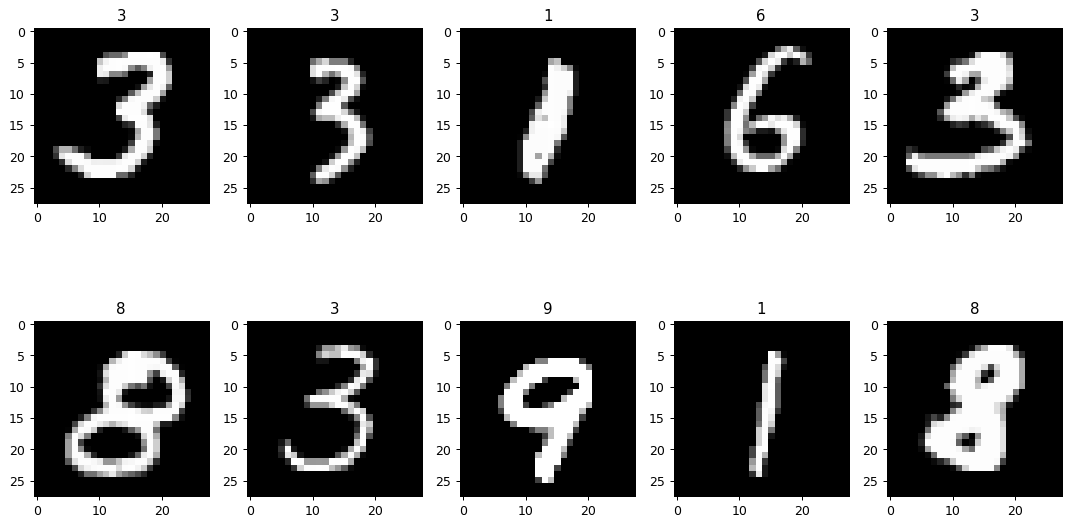
\includegraphics[width=.925\linewidth]{figures/mnist_28x28.png}
		\caption{Original data set of $28 \times 28$ images.}
		\label{fig:mnist_28x28}
	\end{subfigure}%
	\begin{subfigure}{.5\textwidth}
		\centering
		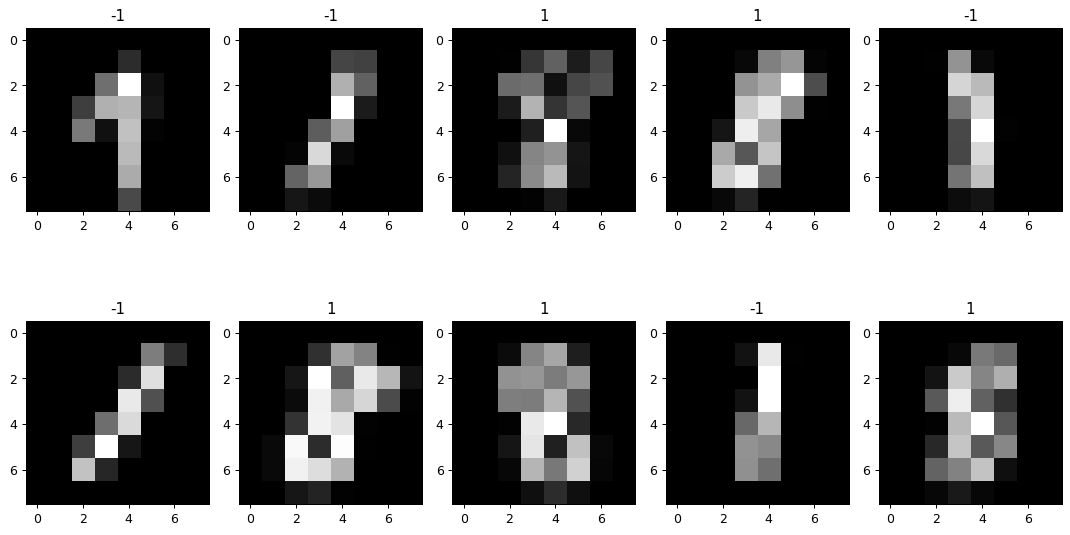
\includegraphics[width=.925\linewidth]{figures/mnist_8x8}
		\caption{Downsampled binary data set of $8 \times 8$ images.}
		\label{fig:mnist_8x8}
	\end{subfigure}
	\caption{Samples of MNIST data set used for classification.}
	\label{fig:mnist}
\end{figure}

\subsubsection{Binary Downsampled Classifier} \label{sec:bdc}
The problem of supervised classification in machine learning is defined as following: given a training set of data whose category is known, train a model which is able to identify to which category new data belongs.
A simple example that we will tackle in this section is recognizing if a handwritten digit is a 1 or an 8.

We implement a QNN to classify $8 \times 8$ images of handwritten digits (Figure~\ref{fig:mnist_8x8}).
It uses a quantum circuit together with a classical optimization algorithm to find the optimal parameters for the quantum circuit.
An overview of the quantum circuit used in the experiment can be found in Figure~\ref{fig:bdc-circuit}.
The variational QNN classifier works as following:
\begin{enumerate}
	\item Prepare data sample $\vec{x}$ in the amplitudes of a quantum state \ket{x}.
	\item Prepare a readout qubit in the state \ket{1}, giving \ket{x, 1}.
	\item Apply $L$ layers of parameterized unitaries: $\mathcal{U}(\vec{\theta})\ket{x, 1}$, where $\mathcal{U}(\vec{\theta}) = U(\vec{\theta}_L) U(\vec{\theta}_{L-1}) \ldots U(\vec{\theta}_1)$.
	\item Measure expectation value $\expval{\sigma_z} = \bra{x, 1}\mathcal{U}(\vec{\theta})^\dagger \sigma_z\, \mathcal{U}(\vec{\theta})\ket{x, 1}$ of readout qubit.
	\item Calculate and minimize loss $\mathcal{L}(\vec{\theta}, \expval{\sigma_z})$ through a classical optimization algorithm.
	\item Repeat until convergence.
\end{enumerate}
\begin{figure}[ht]
	\[
	\Large
	\Qcircuit @C=1em @R=0.4em @!R {
		& & \multigate{5}{U(\vec{\theta}_1)} & \multigate{5}{U(\vec{\theta}_2)} & \qw & & \multigate{5}{U(\vec{\theta}_L)} & \qw & \qw \\
		& & \ghost{U(\vec{\theta}_1)} & \ghost{U(\vec{\theta}_2)} & \qw & & \ghost{U(\vec{\theta}_L)} & \qw & \qw \\
		\lstick{\ket{x}~~} & & \ghost{U(\vec{\theta}_1)} & \ghost{U(\vec{\theta}_2)} & \qw & & \ghost{U(\vec{\theta}_L)} & \qw & \qw \\
		& ~~\vdots & & & ~~\hdots & & & \vdots \\
		& & \ghost{U(\vec{\theta}_1)} & \ghost{U(\vec{\theta}_2)} & \qw & & \ghost{U(\vec{\theta}_L)} & \qw & \qw \\
		& \lstick{\ket{1}} & \ghost{U(\vec{\theta}_1)} & \ghost{U(\vec{\theta}_2)} & \qw & & \ghost{U(\vec{\theta}_L)} & \meter & \rstick{\expval{\sigma_z}} \cw
		\gategroup{1}{1}{5}{1}{.7em}{\{}
	}
	\]
	\caption{General circuit of the QNN\@. The network consists of $L$ layers with each layer implementing a parameterized unitary $U(\vec{\theta})$ whose parameters are optimized using a classical optimization algorithm. At the end of the circuit, the expectation value $\expval{\sigma_z}$ of the readout qubit is measured and the predicted class is decided by $\sign(\expval{\sigma_z})$. The decomposition of a layer is shown in Figure \ref{fig:parametrized_unitary}.}
	\label{fig:bdc-circuit}
\end{figure}

We trained a QNN using a training set of 2014 images and a test set of 843 images.
As optimizer, we used mini-batch stochastic gradient descent (SGD) with a learning rate of $0.4$ and a batch size of $32$.
Due to computational cost, we define one epoch as processing one mini-batch and doing one optimization step, instead of going over the whole training set in batches.
After training for 20 epochs with 2 layers, it managed to reach 91.1\% accuracy without any hyperparameter tuning or circuit optimization.
Note that this means that the network was trained on $32 \cdot 20 = 640$ samples from the original set of 2014 images, due to our one mini-batch per epoch approach.
Ideally we would use true mini-batches, but as we are limited to classical simulation of quantum circuits, this would take a very long time.

The goal of this experiment is not to compete with classical state-of-the-art neural networks, which are capable of achieving an error percentage of only 0.23\%~(\cite{cirecsan2012multi})\footnote{Which is not to say quantum neural networks can't compete with classical neural networks. In fact,~\cite{perez2019data} show a quantum classifier with two qubits to be at least comparable with classical methods.}.
Rather, it is meant to demonstrate the possibility of using quantum computers for machine learning problems and to hint that the universal approximation theorem (\cite{csaji2001approximation}) applies to quantum neural networks.
It shows the potential, given we solve the issues surrounding qRAM~(\cite{aaronson2015read}), to use quantum computers to process (quantum) data which classical computers cannot process efficiently.

\begin{figure}[ht]
	\[
	\Large
	\Qcircuit @C=0.7em @R=0.4em @!R {
		& & \multigate{5}{U(\vec{\theta})} & \qw & & \gate{R_x(\theta_{1, 1})} & \gate{R_y(\theta_{1, 2})} & \gate{R_z(\theta_{1, 3})} & \ctrl{1} & \qw & \qw & \targ & \qw \\
		& & \ghost{U(\vec{\theta})} & \qw & & \gate{R_x(\theta_{2, 1})} & \gate{R_y(\theta_{2, 2})} & \gate{R_z(\theta_{2, 3})} & \targ & \ctrl{1} & \qw & \qw & \qw \\
		& & \ghost{U(\vec{\theta})} & \qw & & \gate{R_x(\theta_{3, 1})} & \gate{R_y(\theta_{3, 2})} & \gate{R_z(\theta_{3, 3})} & \qw & \targ & \qw & \qw & \qw \\
		& & & ~~= & & \vdots & \vdots & \vdots & & \vdots & & & & & \\
		& & \ghost{U(\vec{\theta})} & \qw & & \gate{R_x(\theta_{n-1, 1})} & \gate{R_y(\theta_{n-1, 2})} & \gate{R_z(\theta_{n-1, 3})} & \qw & \qw & \ctrl{1} & \qw & \qw  \\
		& & \ghost{U(\vec{\theta})} & \qw & & \gate{R_x(\theta_{n, 1})} & \gate{R_y(\theta_{n, 2})} & \gate{R_z(\theta_{n, 3})} & \qw & \qw & \targ & \ctrl{-5} & \qw
	}
	\]
	\caption{Decomposition of a layer $U(\vec{\theta})$. The amount of trainable parameters for a QNN with $n$ qubits and $L$ layers is $3n \cdot L$. The amount of qubits required is decided by the dimension of the data: $n = \lceil \log_2N \rceil + 1$, where $N$ is the input dimension. The downsampled MNIST classifier requires $\lceil \log_2(8 \cdot 8) \rceil + 1 = 7$ qubits.}
	\label{fig:parametrized_unitary}
\end{figure}

\subsubsection{One-vs-Rest Classifier}
To make a step into the direction of multi-class classification using a QNN, we first consider the problem of one-vs-rest classification.
We use the original $28 \times 28$ MNIST data set (Figure~\ref{fig:mnist_28x28}) to train a QNN to detect if a handwritten digit is 0 or not 0.
To encode a $28 \times 28$-dimensional image we need $\lceil \log_2(28 \cdot 28) \rceil = 10$ qubits, plus a readout qubit, for $11$ qubits total.
As the complexity of the problem grows, we compare the performance of multiple optimizers: SGD, RMSprop and Adam.
We trained the network for 100 epochs with a batch size of 64.
Some hyperparameter tuning was done to find the optimal learning rate, but more tuning can be done to possibly increase performance.
The results of the experiment are shown in Figure~\ref{fig:ovr_results}.
Increasing the amount of layers seems to improve convergence rate, but ultimately there doesn't seem to be a big performance gain from increasing the amount of layers for this certain problem.
The exception to this is SGD, which seems to benefit from more layers up to 4, after which its performance decreases again.
RMSprop and Adam both seem to converge to around 95\% accuracy, where SGD settles in at 90\%.
\begin{figure}[ht]
	\centering
	\begin{subfigure}{1\textwidth}
		\centering
		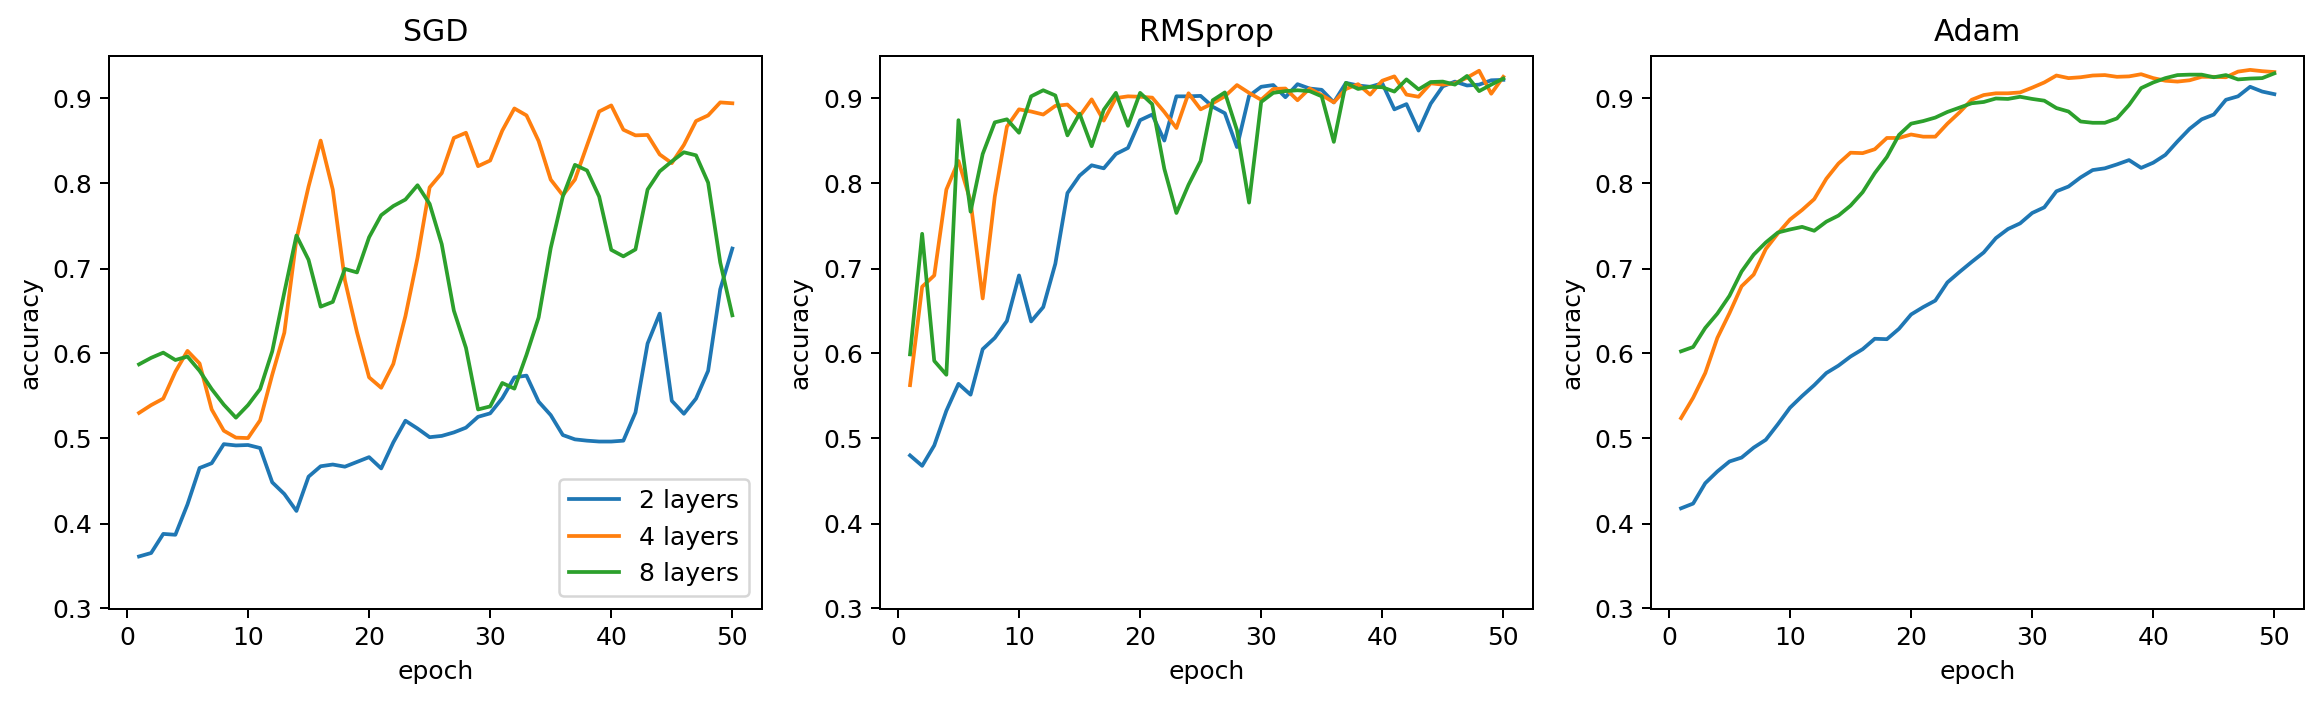
\includegraphics[width=1\linewidth]{figures/qnn_ovr_accuracy.png}
		\caption{Accuracy on test data set with different optimizers.}
		\vspace*{4mm}
	\end{subfigure}
	\begin{subfigure}{1\textwidth}
		\centering
		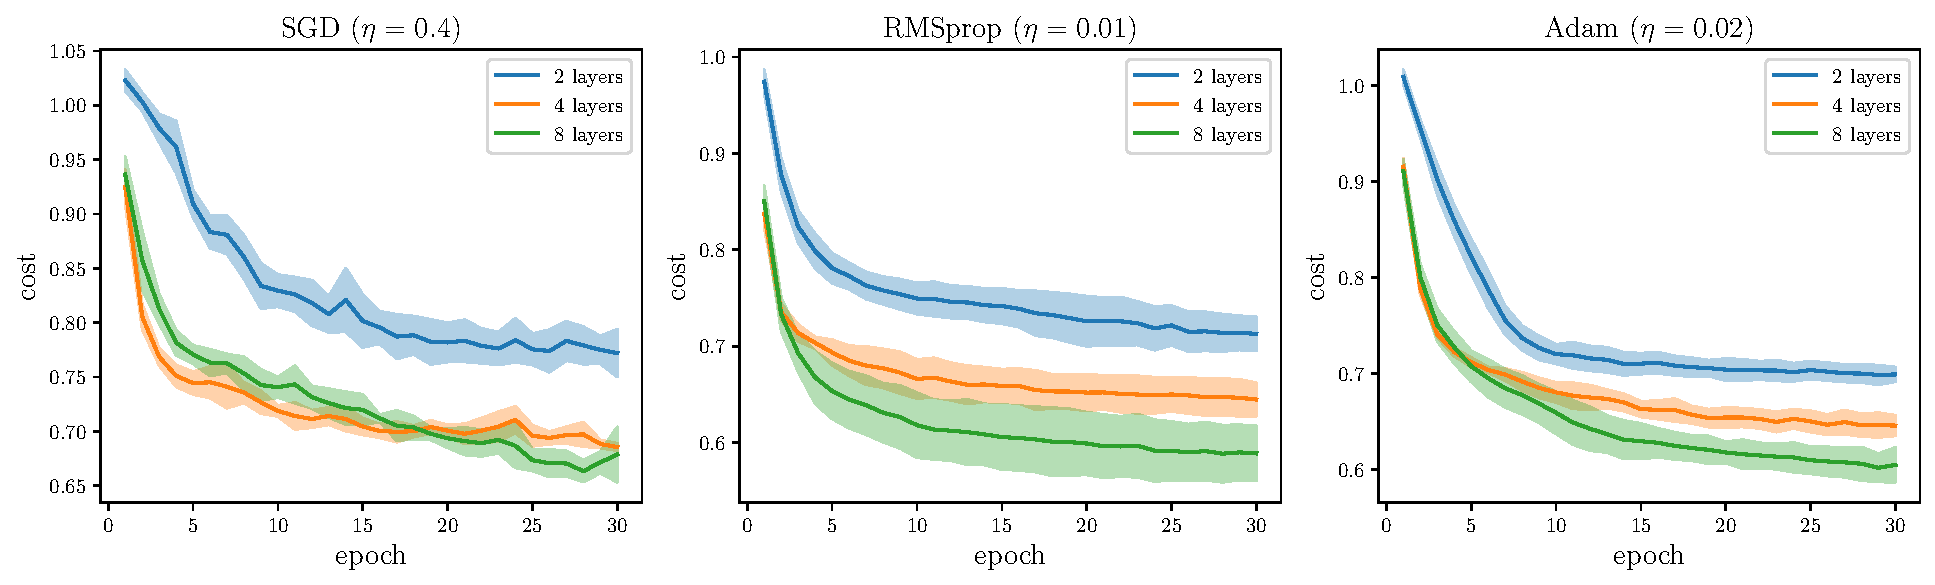
\includegraphics[width=1\linewidth]{figures/qnn_ovr_cost}
		\caption{Cost landscape of different optimizers.}
	\end{subfigure}
	\caption{Experimental results of a one-vs-rest QNN classifier for detecting if a handwritten digit is 0 or not.}
	\label{fig:ovr_results}
\end{figure}

\subsubsection{Multiclass Classifier}
Finally we generalize the QNN to a multiclass classifier by implementing a fidelity loss function as proposed by~\cite{perez2019data}.
To implement this we need to make some changes to the QNN described in Section~\ref{sec:bdc}.
First, we introduce $C$ maximally orthogonal label states, where $C$ is the number of classes (Figure~\ref{fig:orthanogal_label_states}).
Then, instead of using the square loss function on the expectation value as cost, we measure the fidelity of the final state of the readout qubit and the label state.
The goal then is to maximize the fidelity between the final state of the readout qubit and the correct label state.
We define the fidelity cost function as following:
%\begin{equation}
%\mathcal{F}(\vec{\theta}) = \dfrac{1}{D} \sum_{d=1}^{D} \left(1 - \lvert \bra{y_d}\mathcal{U}(\vec{\theta})\ket{x_d, 1} \rvert^2\right),
%\end{equation}
\begin{equation}
\mathcal{F}(\vec{\theta}) = - \dfrac{1}{D} \sum_{d=1}^{D} \log \left( \lvert \bra{y_d}\mathcal{U}(\vec{\theta})\ket{x_d, 1} \rvert^2\right),
\end{equation}
where $D$ is the number of training samples, $\ket{y_d}$ the correct label state of input $\ket{x_d}$, and $\mathcal{U}(\vec{\theta})$ the parameterized circuit unitaries.
We use a negative log likelihood cost function, as the fidelity of quantum states ranges between 0 and 1.

We conduct a similar experiment to that from the previous section.
The problem at hand is to distinguish between the handwritten digits 1 through 6 including, giving six classes.
We take the six polar states $\{\ket{0}, \ket{1}, \ket{+}, \ket{-}, \ket{+i}, \ket{-i}\}$ as our maximally orthogonal label states (Figure~\ref{fig:orthanogal_label_states}).
The network was trained for 200 epochs with a batch size of 32.
The results are shown in Table~\ref{table:multiclass_results}.
\begin{table}[ht]
	\centering
	\begin{minipage}{.49\textwidth}
		\centering
		\contourlength{1.25pt}
		\begin{blochsphere}[radius=1.5cm, tilt=15, rotation=-20, opacity=0.1, color=white]
			\drawBallGrid[style={opacity=0.05}]{30}{30};
			
			\labelLatLon{zero}{90}{0};
			\labelLatLon{min}{0}{180};
			\labelLatLon{mini}{0}{90};
			\labelLatLon{plusi}{180}{90};
			\labelLatLon{plus}{0}{0};
			\labelLatLon{one}{-90}{90};
				
			\drawGreatCircle[style={opacity=0.4}]{0}{0}{0};
			\drawGreatCircle[style={opacity=0.4}]{90}{0}{0};
			\drawGreatCircle[style={opacity=0.4}]{90}{90}{90};
			
			\node[right=1mm] at (plusi) {\ket{+i}};
		
			\draw[opacity=0.4] (min) -- (plus);
			\draw[opacity=0.4] (mini) -- (plusi);
				
			\draw[color=red, line width=0.27mm, opacity=0.7] (zero) -- (plus);
			\draw[color=red, line width=0.27mm, opacity=0.7] (zero) -- (min);
			\draw[color=red, line width=0.27mm, opacity=0.7] (zero) -- (plusi);
			
			\draw[color=red, line width=0.27mm, opacity=0.7] (min) -- (plusi);
			
			\drawStateLatLon[statecolor=blue, statewidth=0.5pt, opacity=1]{state}{103}{-18};
			\node[left] at (state) {\ket{\psi}};
			
			\draw[color=red, line width=0.27mm, opacity=0.7] (zero) -- (mini);
			
			\draw[color=red, line width=0.27mm, opacity=0.7] (plus) -- (plusi);
			\draw[color=red, line width=0.27mm, opacity=0.7] (plus) -- (mini);
		
			\draw[color=red, line width=0.27mm, opacity=0.7] (min) -- (mini);
			
			\draw[color=red, line width=0.27mm, opacity=0.7] (one) -- (min);
			\draw[color=red, line width=0.27mm, opacity=0.7] (one) -- (plus);
			\draw[color=red, line width=0.27mm, opacity=0.7] (one) -- (mini);
			
			\node[above=1mm] at (zero) {\ket{0}};
			\node[left=1mm] at (min) {\ket{-}};
			\node[left] at (mini) {\contour{black!9}{\ket{-i}}};
			\node[right=1mm] at (plus) {\ket{+}};
	
			\node[below=1mm] at (one) {\ket{1}};
		\end{blochsphere}
		\captionof{figure}{Bloch sphere representation of six maximally orthogonal points which are used as labels. The circuit output state \ket{\psi} would get classified to the class corresponding to the label state \ket{0}, as their fidelity $\lvert\ip{0}{\psi}\rvert^2$ is the largest.}
		\label{fig:orthanogal_label_states}
	\end{minipage}
	\hfill
	\begin{minipage}{.45\textwidth}
		\centering
		{\renewcommand{\arraystretch}{1.2}
		\begin{tabular}{ c|c|c } 
			\hline
			Optimizer & Layers & Test accuracy \\
			\hline
			\multirow{3}{5em}{SGD ($\eta = 0.05$)} & 4 & 24.2\% \\ 
			& 8 & 0\% \\ 
			& 10 & 0\% \\
			& 12 & 0\% \\
			\hline
			\multirow{3}{5em}{RMSprop ($\eta = 0.01$)} & 4 & 60.3\% \\ 
			& 8 & 0\% \\ 
			& 10 & 0\% \\
			& 12 & 0\% \\
			\hline
			\multirow{3}{5em}{Adam ($\eta = 0.02$)} & 4 & 56.4\% \\ 
			& 8 & 0\% \\ 
			& 10 & 0\% \\
			& 12 & 0\% \\
			\hline
		\end{tabular}
		}
		\caption{Quantum neural network performance on multiclass classification of six classes.}
		\label{table:multiclass_results}
	\end{minipage}
\end{table}

\section{Conclusion} \label{sec:conclusion}
We have described and implemented a quantum neural network capable of classification.
By applying the QNN to the problem of handwriting recognition, we have demonstrated its capability of doing binary, one-vs-rest and multiclass classification on classical data.
The QNN is able to represent $N$-dimensional classical data in $\log_2N$ qubits and can also potentially learn properties of quantum data.
Further improvements could be made by using more quantum-specific optimization methods~(\cite{stokes2019quantum, sweke2019stochastic}), improving the circuit initialization strategy~(\cite{mcclean2018barren}), conducting more experiments on quantum and classical data, and experimenting with real quantum hardware.

\clearpage

\printbibliography[heading=bibintoc]

\end{document}